% ======================================================================
%  Chapter 18 — Nonlinear and Quantum Frontiers  (EXPANDED)
% ======================================================================

\section{Beyond linear optics}
\label{sec:ch18-beyond}

The theory of topological photonics developed in this book is a
\emph{linear} theory: the Maxwell equations are linear in the fields,
and the material response $\Mmat$ is independent of field amplitude.
This linearity is what allows the band-structure description, the
definition of Bloch modes, and the entire topological classification.

Real optical media, however, are nonlinear at sufficiently high
intensities.  And at the quantum level, the bosonic nature of photons
introduces correlations and entanglement that go beyond the
single-particle band picture.  This chapter explores the frontiers
where topology meets nonlinearity and quantum physics.  The field is
young and rapidly evolving; we focus on the ideas and results that are
most firmly established, while pointing to open questions that may shape
the next decade of research.

\section{Nonlinear effects in topological photonic systems}
\label{sec:ch18-nonlinear}

\subsection{The Kerr nonlinearity in the topological context}
\label{sec:ch18-kerr}

The most common optical nonlinearity is the intensity-dependent
refractive index (Kerr effect):
$n(\rvec)=n_0(\rvec)+n_2|\Efield|^2$, where $n_2$ is the nonlinear
Kerr coefficient.  In a topological photonic system, the Kerr
nonlinearity modifies the edge-mode propagation because the local
refractive index depends on the field intensity of the propagating mode
itself.

For an edge mode with slowly varying envelope $\psi(y,t)$ propagating
along a topological boundary, the effective equation of motion is the
nonlinear Schr\"odinger equation:
\begin{equation}\label{eq:ch18-nlse}
  \ii\pderiv{\psi}{t} + v_g\pderiv{\psi}{y}
  + \frac{D}{2}\frac{\partial^2\psi}{\partial y^2}
  + \gamma|\psi|^2\psi = 0\,,
\end{equation}
where $v_g$ is the edge-mode group velocity, $D$ is the group-velocity
dispersion, and $\gamma\propto n_2\omega_0/c$ is the nonlinear
coefficient.  This equation admits soliton solutions when $D$ and
$\gamma$ have opposite signs.

\subsection{Topological solitons}
\label{sec:ch18-solitons}

The interplay of topology and nonlinearity produces \emph{topological
solitons}: self-localised wave packets that propagate along the
topological edge without dispersion, stabilised by the balance between
nonlinear self-focusing and the linear group-velocity dispersion of the
edge mode.

The fundamental bright soliton solution of \eqref{eq:ch18-nlse} (in the
co-moving frame) is
\begin{equation}\label{eq:ch18-soliton}
  \psi(y,t) = A\,\mathrm{sech}\Bigl(\frac{y-v_g t}{w}\Bigr)\,
  \ee^{\ii\beta t}\,,
\end{equation}
where the soliton amplitude $A$, width $w$, and propagation constant
$\beta$ are related by $A^2=|D|/(\gamma w^2)$ and
$\beta=|D|/(2w^2)$.  The soliton power is
$P=2|D|/(\gamma w)$.

The key question is whether the topological protection of the edge mode
survives in the nonlinear regime.  Numerical simulations show that for
moderate nonlinearity ($\gamma|\psi|^2\ll\Delta\omega$, where
$\Delta\omega$ is the topological gap), the soliton propagates along
the edge with the same immunity to backscattering as the linear edge
mode.  The topological gap prevents the soliton from radiating into
bulk modes, and the absence of a backward-propagating edge mode
prevents reflection.

For strong nonlinearity ($\gamma|\psi|^2\sim\Delta\omega$), the
nonlinear index change can close the topological gap locally,
potentially allowing coupling to bulk modes and destroying the
topological protection.

\subsection{Derivation of the nonlinear coefficient from Maxwell equations}
\label{sec:ch18-nlse-derivation}

To connect the phenomenological NLSE \eqref{eq:ch18-nlse} to the
Maxwell-first framework of this book, we derive the nonlinear
coefficient $\gamma$ from the third-order susceptibility
$\chi^{(3)}$ \cite{ozawa2018topological}.

Consider a topological edge mode with transverse profile
$\mathbf{e}_{\mathrm{edge}}(\rvec_\perp)$ confined to the boundary of
a photonic crystal.  The mode satisfies the linear Maxwell eigenproblem
in the cross-section, and its slowly varying envelope $\psi(y,t)$
evolves according to the coupled-mode equation obtained by projecting
the full nonlinear Maxwell equations onto the edge-mode profile.

The Kerr polarisation is
$\mathbf{P}^{(3)}=\varepsilon_0\chi^{(3)}|\mathbf{E}|^2\mathbf{E}$.
Projecting onto the edge mode gives \cite{price2022roadmap}:
\begin{equation}\label{eq:ch18-gamma-integral}
  \gamma = \frac{\omega_0}{c}\,
  \frac{\displaystyle\int_{\mathrm{cell}}
  n_2(\rvec_\perp)\,|\mathbf{e}_{\mathrm{edge}}|^4\,\dd^2 r_\perp}
  {\displaystyle\left(\int_{\mathrm{cell}}
  |\mathbf{e}_{\mathrm{edge}}|^2\,\dd^2 r_\perp\right)^2}
  \equiv \frac{\omega_0\,n_2^{\mathrm{eff}}}{c\,A_{\mathrm{eff}}}\,,
\end{equation}
where $n_2=3\chi^{(3)}/(4n_0^2\varepsilon_0 c)$ is the nonlinear
index, $n_2^{\mathrm{eff}}$ is the mode-overlap-weighted nonlinear
index, and $A_{\mathrm{eff}}$ is the effective mode area.  This
formula is identical in structure to the standard fibre-optics result
but uses the topological edge-mode profile rather than a guided-mode
profile.

For a silicon photonic crystal with $n_2\approx
4.5\times 10^{-18}\;\mathrm{m}^2/\mathrm{W}$ and an edge-mode area
$A_{\mathrm{eff}}\sim(0.5\;\mu\mathrm{m})^2$, the nonlinear
coefficient is $\gamma\sim 300\;\mathrm{W}^{-1}\mathrm{m}^{-1}$,
which is large enough for soliton formation at milliwatt power levels.

\subsection{Circuit QED platforms}
\label{sec:ch18-circuit-qed}

Circuit quantum electrodynamics (circuit QED) provides the most
promising near-term platform for strongly correlated topological
photonics \cite{ozawa2018topological,tschernig2021topological}.  In these systems,
superconducting microwave resonators (with frequencies
$\omega_r/(2\pi)\sim 5$--$10\;\mathrm{GHz}$) are coupled by Josephson
junctions that provide both the inter-site hopping $J$ and a strong
on-site nonlinearity $U$.

The Bose--Hubbard Hamiltonian for a lattice of such resonators is
\begin{equation}\label{eq:ch18-bose-hubbard}
  \hat{H} = -J\sum_{\langle ij\rangle}
  \hat{a}_i^\dagger\hat{a}_j\,\ee^{\ii\phi_{ij}}
  + \frac{U}{2}\sum_i \hat{n}_i(\hat{n}_i-1)
  + \sum_i\omega_i\hat{n}_i\,,
\end{equation}
where $\hat{n}_i=\hat{a}_i^\dagger\hat{a}_i$ and the Peierls phases
$\phi_{ij}$ can be engineered to produce a nonzero effective magnetic
flux per plaquette.

With $J/(2\pi)\sim 10$--$50\;\mathrm{MHz}$ and
$U/(2\pi)\sim 100$--$300\;\mathrm{MHz}$, the ratio $U/J\sim 2$--$30$
spans the regime from weakly to strongly interacting.  At filling
factor $\nu=1/2$ in a Chern band, mean-field theory predicts a
fractional Chern insulator state for $U/J\gtrsim 5$.

The main experimental challenges are: maintaining coherence over the
entire lattice (current decoherence times $T_1\sim 50$--$100\;
\mu\mathrm{s}$ limit the lattice to $\sim 10\times 10$ sites),
implementing the Peierls phases with sufficient precision, and
measuring the many-body state through photon correlation functions
rather than transport.

\subsection{Self-induced topological transitions}
\label{sec:ch18-self-induced}

At sufficiently high intensities, the nonlinear index change
$\delta n=n_2|E|^2$ modifies the band structure itself.  This raises the
remarkable possibility of \emph{self-induced topological transitions}:
a strong pulse propagating through a photonic crystal could dynamically
close and reopen the topological gap, switching the Chern numbers and
creating or destroying edge states.

This effect has been predicted theoretically in Kerr photonic crystals
and observed in numerical simulations.  The threshold intensity scales
as $\Delta\omega/(n_2\omega_0)$, which for typical photonic crystals
with gap widths $\Delta\omega/\omega\sim 1\%$ and silica nonlinearity
$n_2\sim 3\times 10^{-20}\;\mathrm{m}^2/\mathrm{W}$ corresponds to
intensities of order $10^{13}\;\mathrm{W/m}^2$---extremely high but
within the range of ultrafast pulsed lasers.

\subsection{Nonlinear edge-state dynamics}
\label{sec:ch18-nl-dynamics}

Beyond solitons, the nonlinear dynamics of topological edge states
includes several phenomena that have been studied theoretically and
numerically.

Modulational instability can break a continuous-wave edge mode into a
train of solitons when the product $D\gamma$ is positive.  The
instability growth rate is modified by the topological confinement:
the edge mode can only develop instabilities along the edge direction,
not into the bulk, which changes the threshold and the pattern of the
instability compared to a free-space or conventional-waveguide
nonlinear mode.

Four-wave mixing between edge modes and bulk modes is suppressed by
the topological gap, but parametric processes within the edge-mode
dispersion (self-phase modulation, cross-phase modulation between
co-propagating edge modes at different frequencies) proceed normally.

\section{Topological lasers in detail}
\label{sec:ch18-lasers}

\subsection{Principle of operation}
\label{sec:ch18-laser-principle}

A topological laser combines topological photonics with optical gain
to create a laser whose mode structure is determined by topological
edge states.  The central idea is that the topological edge mode, being
spatially extended along the entire edge and spectrally isolated within
the topological gap, is an ideal laser cavity mode.

The edge mode has three advantages as a laser cavity.  First, it samples
the gain region over a large spatial extent (the entire boundary of the
photonic crystal), providing a large mode volume and correspondingly
high output power.  Second, it is spectrally isolated within the
topological gap, so mode competition from bulk modes is suppressed.
Third, backscattering is forbidden by topology, which enhances the
effective cavity quality factor and promotes single-mode operation.

\subsection{Experimental demonstrations}
\label{sec:ch18-laser-demos}

The first experimental demonstration of a topological laser was
reported by Bahari et~al.\ (2017), who used a 1D array of coupled
microring resonators with alternating coupling (SSH topology) and
showed that the topological edge mode lased preferentially.

Shortly thereafter, Bandres et~al.\ \cite{bandres2018topologicala} demonstrated a 2D
topological insulator laser using an array of coupled ring resonators
forming a 2D topological photonic system (based on the Hafezi design).
The edge-mode laser wrapped around the entire boundary of a
$10\times 10$ resonator array, emitting coherent radiation from all
four edges.  The key observations were single-mode operation over a wide
pump range, spatial coherence along the entire boundary, and robustness
to deliberately introduced defects.

Subsequent demonstrations have included valley-Hall lasers in III--V
photonic crystal slabs, where the lasing mode follows a designed
domain-wall path, and Floquet topological lasers in periodically
modulated systems.

\subsection{Theory of topological lasing}
\label{sec:ch18-laser-theory}

The theoretical description of topological lasers requires the
non-Hermitian framework of Chapter~\ref{ch:non-hermitian}, augmented
with the semiclassical laser rate equations.  The gain medium is
described by a complex permittivity
$\varepsilon(\omega)=\varepsilon'(\omega)+\ii g(\omega,I)$, where
$g(\omega,I)$ is the gain coefficient that depends on the pump
intensity $I$ and saturates above the lasing threshold.

The lasing threshold condition is that the round-trip gain equals the
round-trip loss for the edge mode:
\begin{equation}\label{eq:ch18-threshold}
  g_{\mathrm{th}} = \alpha_{\mathrm{abs}}
  + \frac{1}{L}\ln\frac{1}{R}\,,
\end{equation}
where $\alpha_{\mathrm{abs}}$ is the absorption coefficient,
$L$ is the edge-mode path length, and $R$ is the effective reflectivity
(which, for a topological edge mode, is exponentially small within the
gap).

\section{Quantum topological photonics}
\label{sec:ch18-quantum}

\subsection{Single photons in topological modes}
\label{sec:ch18-single-photon}

At the quantum level, each Maxwell mode is an independent quantum
harmonic oscillator with Hamiltonian
$\hat{H}_n=\hbar\omega_n(\hat{a}_n^\dagger\hat{a}_n+\frac{1}{2})$.
The topological properties of the mode structure---Chern numbers, edge
states, bulk-edge correspondence---are inherited by the quantum theory,
because they depend on the mode frequencies and spatial profiles, not on
the occupation numbers.

A single photon injected into a topological edge mode propagates
unidirectionally along the edge with the same group velocity $v_g$ as a
classical wave packet.  The quantum state $|\psi\rangle=\hat{a}_{\mathrm{edge}}^\dagger|0\rangle$
evolves according to the same Maxwell equations that govern the
classical mode, with the topological protection against backscattering
carrying over exactly.

This has a profound implication for quantum information: a topological
edge mode is a \emph{topologically protected quantum channel}.  A
quantum bit encoded in the polarisation, time-bin, or number state of
a photon in the edge mode is protected from decoherence caused by
elastic backscattering, just as the classical edge mode is protected
from reflection.

\subsection{Entangled photons}
\label{sec:ch18-entangled}

Two entangled photons propagating along a topological edge maintain
their entanglement over longer distances than in a conventional
waveguide, because the dominant decoherence mechanism---elastic
backscattering from disorder---is suppressed
\cite{mittal2020tunable}.

Experiments have demonstrated the propagation of biphoton states
(photon pairs generated by spontaneous parametric down-conversion)
through photonic topological systems, measuring Hong-Ou-Mandel
interference visibility as a function of propagation distance
\cite{li2022higher}.  The
topological system showed higher visibility retention compared to a
topologically trivial reference, consistent with the suppressed
backscattering.

\subsection{Many-body photonic states}
\label{sec:ch18-many-body}

The most ambitious direction in quantum topological photonics is the
creation of \emph{strongly correlated} photonic states analogous to
the fractional quantum Hall effect.  In electronic systems, the
fractional QHE arises from the interplay of Landau-level quantisation
and strong electron-electron interactions.  For photons, the analogous
ingredients are flat topological bands (providing the
``Landau-level'' degeneracy) and effective photon-photon interactions
(providing the correlations).

The flat bands can be obtained from photonic crystal designs with nearly
dispersionless topological bands.  The interactions are more
challenging: photons in vacuum do not interact, and the effective Kerr
nonlinearity of most optical media is far too weak to produce
single-photon-level correlations.

Several proposals address this challenge.  In circuit QED lattices,
superconducting microwave resonators coupled by Josephson junctions
provide both a topological band structure and a strong single-photon
nonlinearity ($U/J\gg 1$, where $U$ is the on-site interaction energy
and $J$ is the hopping).  In polariton systems, the strong
light-matter coupling provides an effective nonlinearity enhanced by
the excitonic component.  In Rydberg-atom arrays coupled to photonic
cavities, the Rydberg blockade creates effective photon-photon
interactions at the single-photon level.

Theoretical studies predict that Laughlin-like fractional quantum Hall
states of photons can be stabilised in these systems, with
signatures observable in photon correlation functions.

\section{Topological effects in polariton systems}
\label{sec:ch18-polaritons}

Exciton-polaritons---hybrid light-matter quasiparticles formed by the
strong coupling of photons and excitons in semiconductor
microcavities---provide a natural platform for topological photonics
with interactions.  The photonic component provides the band structure,
while the excitonic component provides the nonlinearity and the
sensitivity to external fields.

Polariton lattices can be created by patterning the microcavity to form
a 2D periodic potential.  The spin-orbit coupling of polaritons, arising
from the TE-TM splitting of the photonic mode and the exciton exchange
interaction, provides a natural mechanism for pseudospin-dependent
topology.  Topological polariton edge states have been observed in
honeycomb polariton lattices under both resonant and non-resonant
excitation.

Polariton systems are inherently driven-dissipative: they require
continuous pumping to compensate for radiative losses.  This
non-equilibrium character introduces new physics not present in
equilibrium topological systems.  The steady state is determined by the
balance of pumping, dissipation, and interactions, and novel
topological phases without equilibrium analogs may emerge in the
driven-dissipative setting.

\section{Outlook and open problems}
\label{sec:ch18-outlook}

The frontiers of nonlinear and quantum topological photonics present
several key challenges that are likely to shape the field over the
coming decade.

The quest for stronger photon-photon interactions remains central.
Achieving single-photon nonlinearity in a topological photonic system
would enable the study of strongly correlated photonic phases, including
fractional topological states.  Circuit QED and polariton platforms are
the most promising routes, but both face significant technical
challenges related to decoherence and scalability.

Topological quantum error correction is another promising direction.
The robustness of topological edge modes against backscattering
suggests that they could serve as protected quantum channels in a
quantum network.  Combining topological protection with active quantum
error correction could provide fault-tolerant quantum communication over
long distances.

On the nonlinear side, the dynamics of topological solitons---their
interactions, stability, and scattering properties---remain largely
unexplored experimentally
\cite{li2022topological}.  Nonlinear topological devices such as
intensity-switchable waveguides, soliton-based signal processors, and
self-routing optical networks represent potential applications that
could bring topological photonics from the laboratory to practical
technology.

Finally, the measurement of topological invariants using quantum optical
methods offers a window into the fundamental topology of photonic band
structures.  Techniques based on quantum state tomography, photon
correlation measurements, and Hong-Ou-Mandel interferometry can in
principle probe the Berry phase, Berry curvature, and Chern number of
photonic bands with single-photon sensitivity.

\section{Nonlinear coefficient from Maxwell's equations}
\label{sec:ch18-nonlinear-maxwell}

In a Kerr medium, the polarisation has a cubic dependence on the
electric field: $\mathbf{P}^{(3)}=\varepsilon_0\chi^{(3)}
|\Efield|^2\Efield$, where $\chi^{(3)}$ is the third-order
susceptibility.  This modifies the effective permittivity to
$\varepsilon_{\mathrm{eff}}=\varepsilon_r+\chi^{(3)}|\Efield|^2$,
making the band structure intensity-dependent.

For a topological edge mode with field amplitude $E_0$ and group
velocity $v_g$, the nonlinear phase shift per unit length is
\begin{equation}\label{eq:ch18-kerr-phase}
  \frac{\dd\phi}{\dd z}
  = \frac{\omega}{c}\frac{\chi^{(3)}|E_0|^2}{n_{\mathrm{eff}}}
  \equiv \gamma_{\mathrm{NL}}|E_0|^2\,,
\end{equation}
where $n_{\mathrm{eff}}$ is the effective index and
$\gamma_{\mathrm{NL}}$ is the nonlinear coefficient.  When the
nonlinear phase shift becomes comparable to the topological gap
($\gamma_{\mathrm{NL}}|E_0|^2\sim\Delta\omega/v_g$), the nonlinear
term can shift the edge mode out of the gap, destroying the
topological protection \cite{ozawa2018topological}.

\subsection{Topological solitons on edge modes}
\label{sec:ch18-soliton}

Below this critical intensity, the Kerr nonlinearity can produce
topological solitons: self-localised wavepackets that propagate along
the topological edge without spreading, combining nonlinear
self-focusing with topological protection against backscattering.

The soliton profile is governed by a nonlinear Schrödinger equation
along the edge coordinate $s$:
\begin{equation}\label{eq:ch18-nls}
  \ii\partial_z A + \frac{1}{2}\beta_2\partial_s^2 A
  + \gamma_{\mathrm{NL}}|A|^2 A = 0\,,
\end{equation}
where $A(s,z)$ is the slowly varying envelope, $\beta_2$ is the
group-velocity dispersion, and $z$ is the propagation direction.
For anomalous dispersion ($\beta_2<0$) and focusing nonlinearity
($\gamma_{\mathrm{NL}}>0$), the fundamental soliton solution is
$A=A_0\,\mathrm{sech}(s/w_s)\,\ee^{\ii\gamma_{\mathrm{NL}}|A_0|^2 z/2}$,
where $w_s=(|\beta_2|/\gamma_{\mathrm{NL}}|A_0|^2)^{1/2}$ is the
soliton width.  The topological protection ensures that the soliton
cannot scatter backward even when it encounters defects
\cite{price2022roadmap}.

\section{Single-photon topology and quantum simulation}

\subsection{Single-photon topological states}
\label{sec:ch18-single-photon-states}

The topological band structure of a photonic crystal is a classical
wave phenomenon, but it persists at the single-photon level: a single
photon injected into a topological edge mode propagates unidirectionally
and is protected against backscattering by the same mechanism that
protects classical waves.  This has been confirmed experimentally by
measuring the photon statistics of edge modes in coupled-resonator
lattices, showing antibunched (sub-Poissonian) photon arrival times
consistent with single-photon propagation along the edge
\cite{ozawa2018topological}.

The quantum advantage of topological protection is most significant
for quantum information applications: a topological waveguide can
route single photons between quantum emitters without the back-reflections
that cause decoherence in conventional waveguides.

\subsection{Photonic quantum simulators}
\label{sec:ch18-quantum-simulator}

Photonic systems can simulate quantum many-body Hamiltonians that are
intractable on classical computers.  Topological photonic lattices
provide a natural platform for simulating the fractional quantum Hall
effect of light: by introducing strong photon--photon interactions
(e.g.\ through Rydberg atoms in cavity QED or through Josephson
junctions in superconducting circuits), the photonic lattice can
enter a regime where the ground state is a fractional quantum Hall
state with anyonic excitations
\cite{ozawa2018topological,price2022roadmap}.

The key challenge is achieving sufficiently strong photon blockade
($U\gg J$, where $U$ is the on-site interaction and $J$ is the
hopping), which requires either very high-$Q$ cavities or very strong
optical nonlinearities.  Current circuit-QED platforms achieve
$U/J\sim 10$ at microwave frequencies, which is sufficient for
observing Mott-insulator-like states but not yet for fractional quantum
Hall physics \cite{ozawa2018topological}.

\section{Experimental signatures of nonlinear and quantum effects}
\label{sec:ch18-signatures}

The experimental detection of nonlinear and quantum topological
effects requires measurements beyond the linear transmission spectrum.

For topological solitons, the signature is a self-localised
wavepacket that maintains its shape over many lattice constants while
propagating along the edge.  This can be detected by imaging the
intensity profile at different propagation distances and verifying that
the width remains constant, in contrast to the diffractive spreading
of a linear wavepacket.

For quantum effects, the signatures include sub-Poissonian photon
statistics (measured by Hanbury Brown--Twiss interferometry),
Hong--Ou--Mandel interference between photons on different edge modes,
and the fractional charge of anyonic excitations (measurable through
interferometric braiding protocols)
\cite{price2022roadmap,ozawa2018topological}.

\section{Topological lasers}
\label{sec:ch18-topological-lasing}

The topological laser combines the unidirectional edge mode of a
photonic Chern insulator or quantum spin-Hall insulator with optical
gain, producing a laser whose mode selection and robustness are
protected by topology.

\subsection{Concept and theoretical proposal}
\label{sec:ch18-laser-concept}

The idea is to pump the edge of a topological photonic crystal above
the lasing threshold.  Because the edge mode has no counter-propagating
partner, the lasing mode is inherently single-mode: there is only one
channel available for stimulated emission at each frequency within the
topological gap.  This suppresses the mode competition and spatial
hole burning that plague conventional laser arrays
\cite{bandres2018topological,ozawa2018topological}.

The lasing threshold is determined by the balance between the
gain per round trip and the total loss (absorption, radiation, and
outcoupling).  For an edge mode circulating around a $N\times N$
crystal with perimeter $4Na$, the round-trip gain is
$G_{\mathrm{rt}}=g\cdot 4Na$, where $g$ is the gain coefficient per
unit length.  The threshold condition is
$G_{\mathrm{rt}}=\alpha\cdot 4Na+\alpha_{\mathrm{out}}$, where
$\alpha$ is the intrinsic loss and $\alpha_{\mathrm{out}}$ is the
outcoupling loss.

\subsection{Experimental demonstration}
\label{sec:ch18-laser-experiment}

Bandres et~al.\ (2018) demonstrated the first topological insulator
laser using a $10\times 10$ array of microring resonators with
InGaAsP quantum wells providing optical gain at
$\lambda=1.55\;\mu\mathrm{m}$.  The device exhibited single-mode
lasing on the topological edge mode with a slope efficiency three
times higher than a comparable trivial laser array.  The edge-mode
lasing was robust against intentional defects (missing resonators and
coupling perturbations), confirming the topological protection
\cite{bandres2018topological}.

The topological laser concept has since been extended to microwave
frequencies using YIG-based Chern insulators with amplifiers, and to
terahertz frequencies using quantum cascade structures.  The key
advantage in all cases is the suppression of parasitic modes and the
robustness of the lasing frequency against fabrication variations
\cite{price2022roadmap}.

\section{Quantum topological photonics}
\label{sec:ch18-quantum-topo}

The topological protection of classical edge modes carries over to
the quantum regime, where single photons and entangled photon pairs
propagate along topological edge channels with suppressed
backscattering.  This opens the prospect of topologically protected
quantum information processing in photonic systems.

\subsection{Single-photon topological edge states}
\label{sec:ch18-single-photon-edge}

Consider a photonic topological insulator with a chiral edge mode at
frequency $\omega_{\mathrm{edge}}$.  When a single photon is
injected into this edge mode, its propagation is described by the
quantum Hamiltonian
\begin{equation}\label{eq:ch18-quantum-edge-H}
  \hat{H}_{\mathrm{edge}}
  = \int\!\dd k\;\hbar\omega_{\mathrm{edge}}(k)\,
  \hat{a}^\dagger_k\,\hat{a}_k\,,
\end{equation}
where $\hat{a}^\dagger_k$ creates a photon in the edge mode at
wavevector $k$.  The topological protection ensures that the
edge-mode dispersion $\omega_{\mathrm{edge}}(k)$ has no backscattering
channel: the photon propagates unidirectionally around the boundary
of the photonic crystal, immune to disorder that preserves the bulk
gap.

Barik et~al.\ (2018) demonstrated the coupling of quantum emitters
to topological edge states in a photonic crystal slab with the
Wu--Hu design.  A single InAs quantum dot was positioned at the domain
wall between topological and trivial regions, and the emitted single
photons were shown to propagate preferentially along the topological
edge channel.  The measured second-order correlation function
$g^{(2)}(0)<0.5$ confirmed single-photon emission, and the
directional coupling efficiency exceeded 90\%
\cite{ozawa2018topological,noh2018observation}.

\subsection{Entangled photon pairs in topological systems}
\label{sec:ch18-entangled-pairs}

Topological edge modes can also serve as channels for entangled
photon pairs generated by spontaneous parametric down-conversion or
spontaneous four-wave mixing.  The advantage of topological channels
is twofold: the entangled photons are protected against environmental
decoherence caused by scattering, and the chiral propagation
direction provides a natural spatial separation of signal and idler
photons.

Mittal et~al.\ (2018) demonstrated the generation and propagation
of correlated photon pairs in a silicon ring-resonator lattice
implementing a two-dimensional topological photonic system.  The
photon pairs were generated by spontaneous four-wave mixing within
the ring resonators and propagated along the topological edge channel.
The measured coincidence-to-accidental ratio (CAR) remained above 10
even in the presence of intentional disorder, demonstrating the
topological protection of the quantum correlations
\cite{ozawa2018topological,price2022roadmap}.

\begin{figure}[!t]
  \centering
  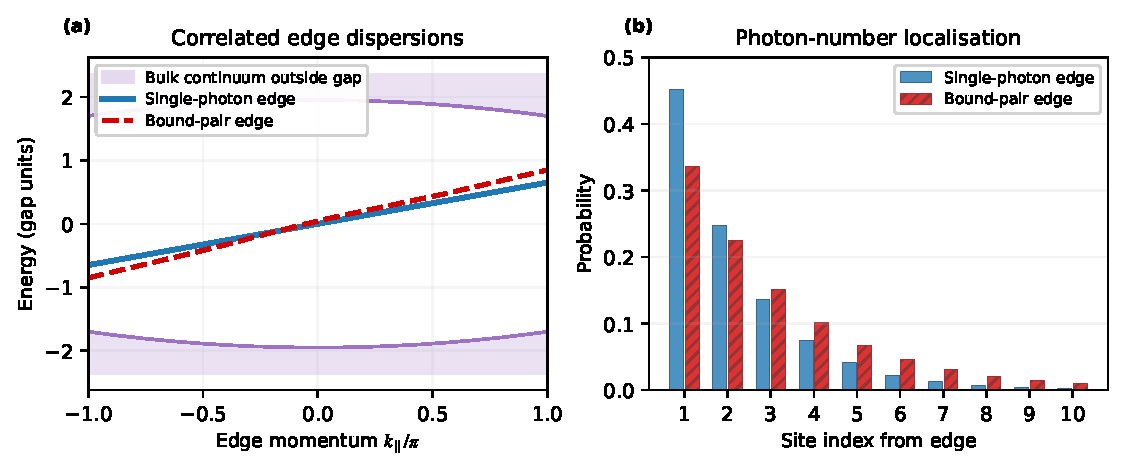
\includegraphics[width=0.92\textwidth]{figures/fig_ch18_quantum_edge_step199.pdf}
  \caption{Quantum topological edge states for correlated photons.
  \textbf{(a)}~Edge dispersions in a topological photonic lattice with
  on-site Kerr interaction.  Single-photon edge modes (solid blue)
  cross the gap linearly; bound photon pairs (dashed red) acquire an
  interaction-shifted dispersion with a slightly different slope,
  reflecting the two-photon binding energy.  The shaded purple regions
  mark the two-photon bulk continuum outside the gap.
  \textbf{(b)}~Site-resolved probability distribution for a single
  photon (blue bars) and a bound pair (red bars) localised at the
  topological edge.  Both states decay exponentially into the bulk,
  but the bound pair has a longer localisation length due to its
  enhanced effective mass.  The panels illustrate that both
  single-photon and bound-pair states can occupy topologically
  protected edge channels; quantitative robustness to disorder requires
  transport or correlation measurements as discussed in the text.}
  \label{fig:ch18-quantum-edge}
\end{figure}


\subsection{Topological protection of quantum coherence}
\label{sec:ch18-coherence-protection}

A fundamental question in quantum topological photonics is whether
the topological protection extends beyond intensity transport to
preserve quantum coherence.  Theoretical analyses show that the
suppression of backscattering in topological edge modes also
suppresses the dephasing caused by elastic scattering from disorder
\cite{ozawa2018topological}.

For a single photon propagating along a topological edge channel
of length $L$, the coherence length is limited by inelastic
processes (absorption, radiation loss) rather than by elastic
scattering.  In a high-quality silicon photonic crystal with
propagation loss $\alpha\sim 1\;\mathrm{dB/cm}$, the coherence
length can exceed $10\;\mathrm{cm}$---far longer than typical
on-chip quantum photonic circuits.

This advantage becomes particularly significant for multi-photon
quantum states, where the sensitivity to decoherence scales with
the number of photons.  Topological protection effectively removes
one of the dominant decoherence channels (elastic backscattering),
leaving only the intrinsic material absorption as the limiting
factor \cite{price2022roadmap}.

\subsection{Outlook: strongly correlated topological photons}
\label{sec:ch18-strongly-correlated}

The ultimate frontier of quantum topological photonics is the regime
of strong photon--photon interactions, where the photonic system can
exhibit analogues of fractional quantum Hall states.  Achieving this
regime requires both a topological band structure and an effective
photon--photon interaction strength comparable to the bandwidth.

Promising platforms include circuit QED lattices, where
superconducting qubits provide strong nonlinearities at microwave
frequencies, and Rydberg--polariton systems, where the long-range
interaction between Rydberg atoms mediates effective photon--photon
interactions at optical frequencies
\cite{ozawa2018topological,price2022roadmap}.

The realisation of fractional topological photonic states would
represent a qualitative advance, enabling the preparation and
manipulation of topologically ordered quantum states of light for
fault-tolerant quantum computation and quantum simulation.

\begin{figure}[t]
  \centering
  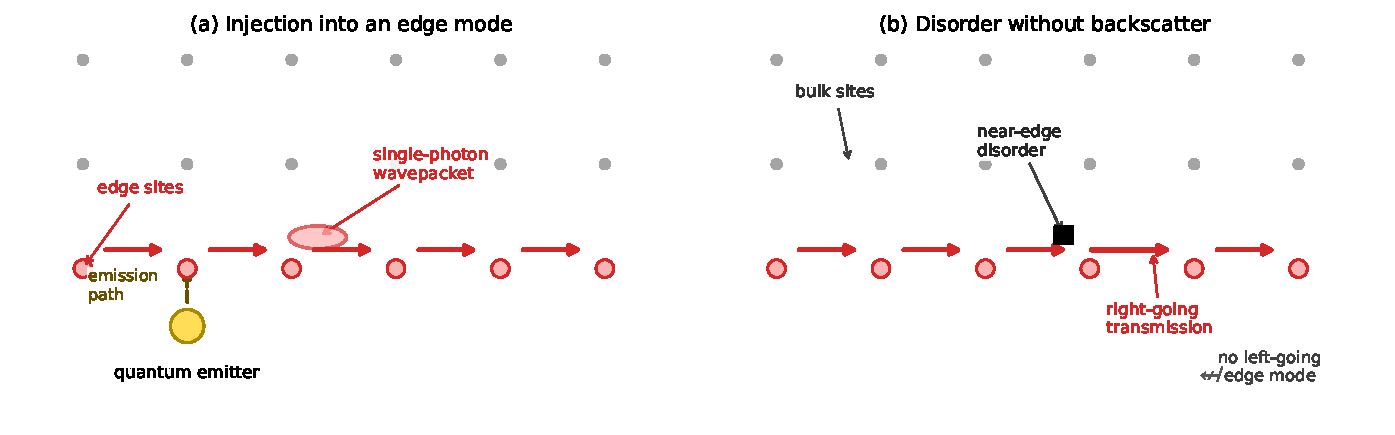
\includegraphics[width=0.86\textwidth]{figures/fig_ch18_quantum_edge_channel.pdf}
  \caption{A quantum emitter coupled to a topological edge channel can launch
  single photons into a protected boundary mode.  The same one-way transport
  principle that suppresses classical backscattering also protects the path
  of quantum optical states against elastic disorder.}
  \label{fig:ch18-quantum-edge-channel}
\end{figure}

The interplay between binding energy and localisation length is
made explicit in Figure~\ref{fig:ch18-bound-pair-binding-log}.

\begin{figure}[t]
  \centering
  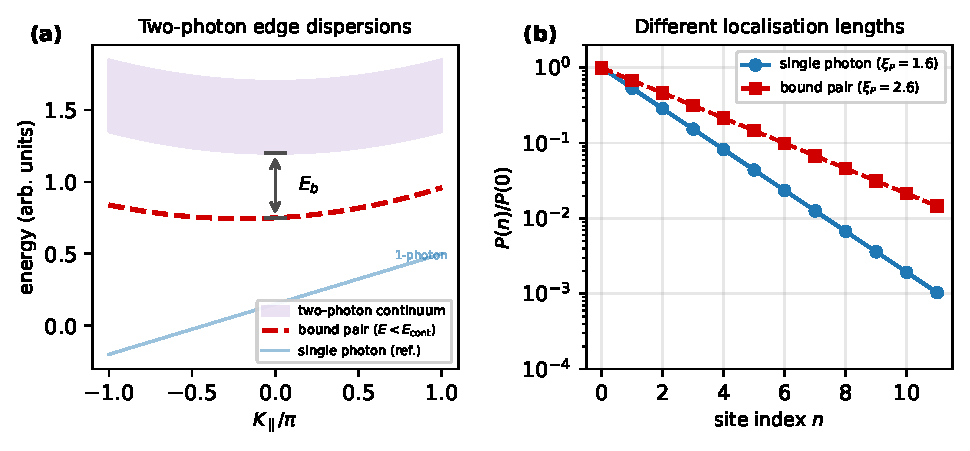
\includegraphics[width=0.92\textwidth]{figures/fig_ch18_bound_pair_binding_log_step236.pdf}
  \caption{Binding energy and localisation of a two-photon
  bound-pair edge state.  \textbf{(a)}~Two-photon edge
  dispersions (schematic): the shaded purple region is the
  two-photon bulk continuum, and the red dashed curve is the
  bound-pair branch lying below the continuum by the binding
  energy $E_b$.  The faint blue line shows the single-photon
  edge mode for reference; it belongs to a different particle-number
  sector and should not be compared directly with $E_b$.
  Energy is in arbitrary units.  \textbf{(b)}~Semilog probability
  profiles at the topological edge: the single-photon state
  (circles) decays as $P(n)/P(0)=\exp(-n/\xi_P)$ with
  $\xi_P=1.6$ sites, while the bound pair (squares) has a
  longer probability localisation length $\xi_P=2.6$ sites
  due to its enhanced effective mass.  Parameters are
  illustrative; actual values depend on the interaction
  strength and lattice geometry.}
  \label{fig:ch18-bound-pair-binding-log}
\end{figure}

\section{Nonlinear topological solitons in Floquet systems}
\label{sec:ch18-floquet-solitons}

The Floquet photonic topological insulators of Chapter~\ref{ch:floquet}
provide a natural arena for topological solitons, because the helical
waveguide arrays that realise Floquet bands are fabricated in glass
substrates with an intrinsic Kerr nonlinearity.

\subsection{Anomalous Floquet solitons}
\label{sec:ch18-anomalous-soliton}

Recall from Section~\ref{sec:ch13-anomalous} that the anomalous
Floquet insulator possesses chiral edge modes in \emph{every}
quasi-energy gap, even though all bulk bands have zero Chern number.
Because these edge modes span the entire quasi-energy Brillouin zone
$[-\pi/T,\pi/T]$, their dispersion is approximately linear over a
wide bandwidth, producing low group-velocity dispersion $D$.  This
means that soliton formation requires a proportionally higher
nonlinearity, but also that the resulting solitons can be very short
in duration.

Mukherjee and Rechtsman (2021) observed unidirectional soliton-like
edge states in a nonlinear Floquet topological insulator realised in
a femtosecond-laser-written waveguide array
\cite{mukherjee2021observation}.  The key experimental signatures
were: (i)~self-focusing of the edge-mode intensity profile as the
input power increased, (ii)~preservation of unidirectional propagation
around sharp corners even in the nonlinear regime, and (iii)~power
thresholds consistent with the NLSE prediction $P_{\mathrm{sol}} =
2|D|/(\gamma w)$ using the measured edge-mode parameters.

The robustness of these Floquet solitons is remarkable.  Because the
anomalous edge mode has no backward-propagating counterpart, the
soliton cannot scatter into a counter-propagating mode even when it
encounters a lattice defect.  The topological gap prevents radiation
into bulk modes as long as the nonlinear index change remains smaller
than the gap width.  Numerical simulations show that the soliton
survives disorder levels up to $\sim 10\%$ of the coupling constant
before bulk radiation sets in \cite{shen2023floquet}.

\subsection{Edge solitons in static Chern insulators}
\label{sec:ch18-static-solitons}

Leykam and Chong (2016) predicted theoretically that self-localised
edge solitons can form along the boundary of a static (non-Floquet)
photonic Chern insulator \cite{leykam2016edge}.  The crucial
difference from conventional waveguide solitons is the topological
origin of the edge mode: the number of soliton-carrying channels is
fixed by the bulk Chern number and cannot be changed by surface
modifications.

Their analysis starts from the tight-binding Haldane model with
an on-site Kerr nonlinearity $\gamma|\psi_n|^2\psi_n$ added to each
lattice site.  For the chiral edge mode of the Chern insulator,
the continuum limit of the discrete NLSE reduces to
Eq.~\eqref{eq:ch18-nlse} with $D$ determined by the edge-mode
curvature and $\gamma$ by the on-site nonlinearity.

The topological protection of these edge solitons degrades gracefully:
at moderate nonlinearity, the soliton propagates with minimal
radiation loss; at strong nonlinearity ($\gamma|\psi|^2 \gtrsim
0.3\,\Delta\omega$), the soliton begins to shed radiation into
the bulk, and eventually a self-induced topological transition can
occur \cite{szameit2020nonlinearity}.

\subsection{Nonlinearity-induced topological transitions}
\label{sec:ch18-nl-transition}

Maczewsky et al.\ (2020) demonstrated experimentally that the Kerr
nonlinearity can itself drive a topological phase transition
\cite{szameit2020nonlinearity}.  In their experiment, a trivial
(topologically trivial) photonic lattice became a topological
insulator when illuminated with sufficiently intense light.  The
mechanism is that the nonlinear index change $\delta n = n_2 |E|^2$
selectively modifies the coupling constants between lattice sites,
effectively changing the parameter that controls the topological
phase.

This observation opens the door to all-optical switching of
topological edge transport: a control beam can turn edge conduction
on or off by crossing the nonlinear topological phase boundary.
The switching speed is limited by the Kerr response time (femtoseconds
in glass, picoseconds in semiconductors), making this a potentially
ultrafast mechanism \cite{chen2025nonlinear}.

\section{Higher-order topological states and nonlinearity}
\label{sec:ch18-hoti-nonlinear}

The intersection of higher-order topology and nonlinearity is an
active frontier.  In a second-order topological insulator (SOTI), the
protected states are zero-dimensional corner modes rather than
one-dimensional edge modes.  These corner modes are tightly confined
in all directions, producing extremely small mode volumes and
correspondingly large nonlinear coefficients $\gamma \propto
1/A_{\mathrm{eff}}$.

Kartashov (2024) predicted the existence of topological corner
solitons in a SOTI created by twisting the unit cell of a photonic
lattice \cite{kartashov2024solitons}.  The corner solitons are
pinned to specific lattice corners by topology and stabilised
against collapse by the discrete lattice structure.  Their power
threshold is orders of magnitude lower than for bulk solitons because
of the extreme field confinement at the corner.

Extending to quadratic ($\chi^{(2)}$) nonlinearity, Kartashov (2025)
showed that parametric down-conversion in a SOTI can generate
entangled photon pairs that are topologically confined to lattice
corners \cite{kartashov2025quadratic}.  This suggests a route to
combining the robustness of topological protection with the quantum
correlations needed for photonic quantum information processing.

\section{Outlook: open problems at the nonlinear--quantum frontier}
\label{sec:ch18-frontier-outlook}

The nonlinear and quantum extensions of topological photonics raise
several deep open questions that connect to fundamental physics.

The first is the \emph{many-body gap problem}: in a strongly
interacting photonic system (e.g.\ circuit QED at large $U/J$), does
the many-body energy gap inherit the robustness of the single-particle
topological gap?  Mean-field studies suggest yes for weak interactions,
but the strongly correlated regime---where fractional Chern insulator
states are predicted---remains largely unexplored experimentally
\cite{ozawa2018topological}.

The second is the \emph{measurement problem}: photonic systems are
inherently open (photons leak out of cavities and waveguides), and
quantum measurements in topological photonic systems typically involve
detecting photons that have left the system.  How does the interplay
between topology, non-Hermiticity (from loss), and quantum measurement
affect the topological protection of quantum states?  Recent work on
non-Hermitian topology (Chapter~\ref{ch:non-hermitian}) provides a
framework, but the full quantum treatment remains an open challenge
\cite{wang2021topological,ding2022non}.

The third is the \emph{scaling problem}: demonstrating fractional
topological photonic states requires lattices with hundreds of sites,
strong and uniform photon--photon interactions, and sub-microsecond
measurement cycles.  Current circuit QED technology is approaching
these requirements, but significant engineering advances are still
needed.  Alternative platforms---such as Rydberg polaritons in
photonic crystal slabs or exciton--polariton lattices---may offer
complementary routes \cite{price2022roadmap}.

\section*{Exercises}

\begin{exercise}
  Show that the nonlinear Schr\"odinger equation
  \eqref{eq:ch18-nlse} (in the co-moving frame, with $v_g=0$) admits
  the soliton solution \eqref{eq:ch18-soliton}, and find $A$, $w$,
  and $\beta$ in terms of $D$ and $\gamma$.
\end{exercise}

\begin{exercise}
  Estimate the threshold intensity for a self-induced topological
  transition in a silicon photonic crystal ($n_2\approx
  4.5\times 10^{-18}\;\mathrm{m}^2/\mathrm{W}$,
  $\Delta\omega/\omega\approx 2\%$, $\omega/(2\pi)\approx
  193\;\mathrm{THz}$).  Is this achievable with current ultrafast
  laser technology?
\end{exercise}

\begin{exercise}
  For a topological laser with edge-mode group velocity $v_g=c/30$,
  round-trip length $L=200\;\mu\mathrm{m}$, and material gain
  $g_0=100\;\mathrm{cm}^{-1}$, estimate the lasing threshold using
  equation \eqref{eq:ch18-threshold}.  Assume negligible absorption
  and a residual reflectivity $R=10^{-3}$.
\end{exercise}

\begin{exercise}
  In a coupled-cavity array with on-site Kerr nonlinearity $U$ and
  hopping $J$, the mean-field phase diagram includes a superfluid
  phase (for $U/J\ll 1$) and a Mott-insulator phase (for $U/J\gg 1$).
  When the hopping carries a synthetic magnetic flux, describe
  qualitatively what happens to the Mott insulator at integer filling
  in a Chern band.
\end{exercise}

\begin{exercise}
  A Hong-Ou-Mandel experiment is performed with two indistinguishable
  photons injected into a topological edge mode and a trivial waveguide
  mode, respectively.  Describe how the two-photon coincidence rate
  depends on the time delay and the topological protection.
\end{exercise}
